\chapter{Behavior Modeling}
\label{ch:behavior}
% ##################################################################################################################

\hfill \textbf{Author:} Andreas Horni

\begin{center} \includegraphics[width=0.45\textwidth, angle=0]{understanding/figures/acapulco.png} \end{center}

% ##################################################################################################################
\section{Unobserved Heterogeneity and Randomness in the Human Decision Processes}
\ah{
Übliche $\rho^2$s in social science and economical models diskutieren

Was heisst das für die Simulation 
-> link zu Monte Carlo engine chapter
-> link zu variability chapter

unobserved heterogeneity / max entropy 

}

\ah{
Figure \ref{fig:acapulco}
Even if you knew everything about the rational decision determinants, you would still need an $\epsilon$ > 0.5 because it actually IS random. it is all about community. everybody has his own better TV at home, could sit closer and consume beer cheaply.

}

% ------------
\createfigure%
{Rational Choice}%
{Rational Choice}%
{\label{fig:acapulco}}%
{\includegraphics[width=0.99\textwidth, angle=0]{figures/acapulco.png}}%
{}

% ------------

% ##################################################################################################################
\section{Micro-Motives}
\ah{
Akkumulation von Microbiases zu large Bias. Aber jeweilige Micromotives weit unter Modellauflösung. Aggregiert gibt es keinen offensichtlichen Zugang.
}

Even in very large scenarios, small random fluctuations, create an aggregate limit for model improvement. Even if we know all the micro-motives, we also need to know \emph{when} these are triggered. The small-scale fluctuations triggered by micro-motives might not average out, but potentially add up to a substantial bias. A very simple example taken from the author's daily life is shown in Figure \ref{fig:migrosEasy}. The grocery store, marked with a red circle, lies directly at an important distributor road with many commuters and provides competitive prices and free and nearby parking. It covers the common and popular Migros product range and additionally special local products are available, generating a plus in attractiveness. However, Figure \ref{fig:migrosDifficult} shows why the store and in particular its parking lots are much less frequented than supposed considering above advantages. Even the author often passes the store although it is perfectly located at his work route. If the signal-light for the oncoming lane shows green, very dense traffic makes it very uncomfortable to turn left and cross the line. A traffic jam results on the own lane. If there were parking lots on both sides of the road, the store might enjoy up to 50\% load increase. Elimination of these kind of biases in the model would require a too high detail level, meaning that the modeling error is irreducible at some point of the exercise, where this stopping point may come sooner than one usually expects.


% ----------------------
\createfigure%
{Micro-motives and macro-scale biases}%
{Micro-motives and macro-scale biases}%
{\label{fig:hstp}}%
{%
 \createsubfigure%
  {Easy turn}%
  {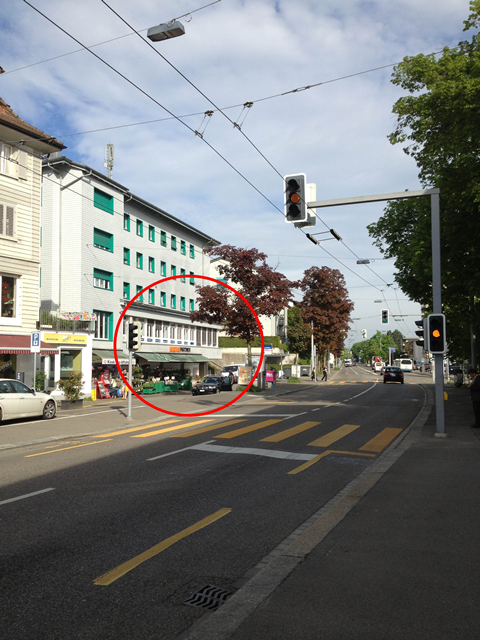
\includegraphics[width=0.49\textwidth]{understanding/figures/IMG_3617.png}}%
  {\label{fig:migrosEasy}}%
  {}%
  \createsubfigure%
  {Uncomfortable turn}%
  {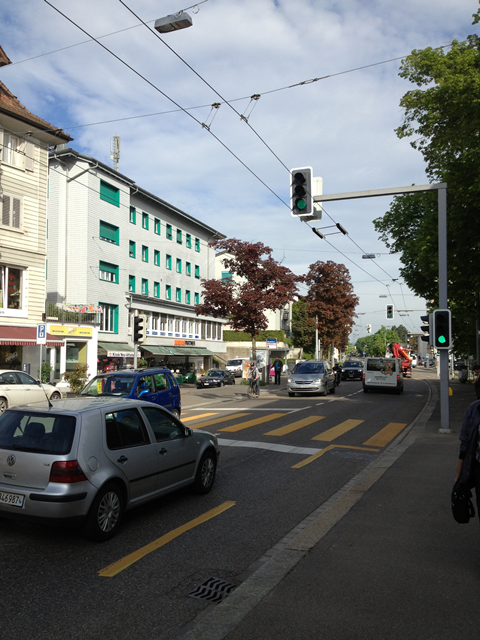
\includegraphics[width=0.49\textwidth]{understanding/figures/IMG_3616.png}}%
  {\label{fig:migrosDifficult}}%
  {}%
}%
{}

% ----------------------

% ##################################################################################################################


